\section{Bonus exercices}
\subsection{Polynomial evaluation using Horner's method}

There exists multiple ways to evaluate polynomials, using associativity, commutativity and factorization.
Each evaluation scheme has its own impact on precision and performance.
One of them has already been the subject of many studies: the Horner's method which for the considered polynomial takes the following form:

\[
  T(x) = (\dots((a_n\times x^2 + a_{n-1})\times x^2 + a_{n-2})\dots) \times x^2
  + a_0
\]

$$T(x) = (((((((((524288*x^2-2621440)*x^2+5570560)*x^2-6553600)*$$
$$x^2+4659200)*x^2-2050048)*x^2+549120)*x^2-84480)*$$
$$x^2+6600)*x^2-200)*x^2+1$$

\begin{question}
  \begin{enumerate}[(a)]
    \item Open the file {\tt tchebychev.c} and have a look to the function {\tt REAL horner(REAL x)}
    \item While keeping previous execution parameters, execute the command {\tt ./run.sh HORNER DOUBLE 53 mca}  \newline The output of this command is given in table~\ref{fig:hor_24_53} (Left).
  \end{enumerate}
\end{question}

\begin{question}
  \item Execute the command {\tt ./run.sh HORNER DOUBLE 24 mca}  \newline
  The output of this command is given in table~\ref{fig:hor_24_53} (Right).
  What do you observe?
\end{question}

\begin{table}
  \begin{tabular}{cc}
    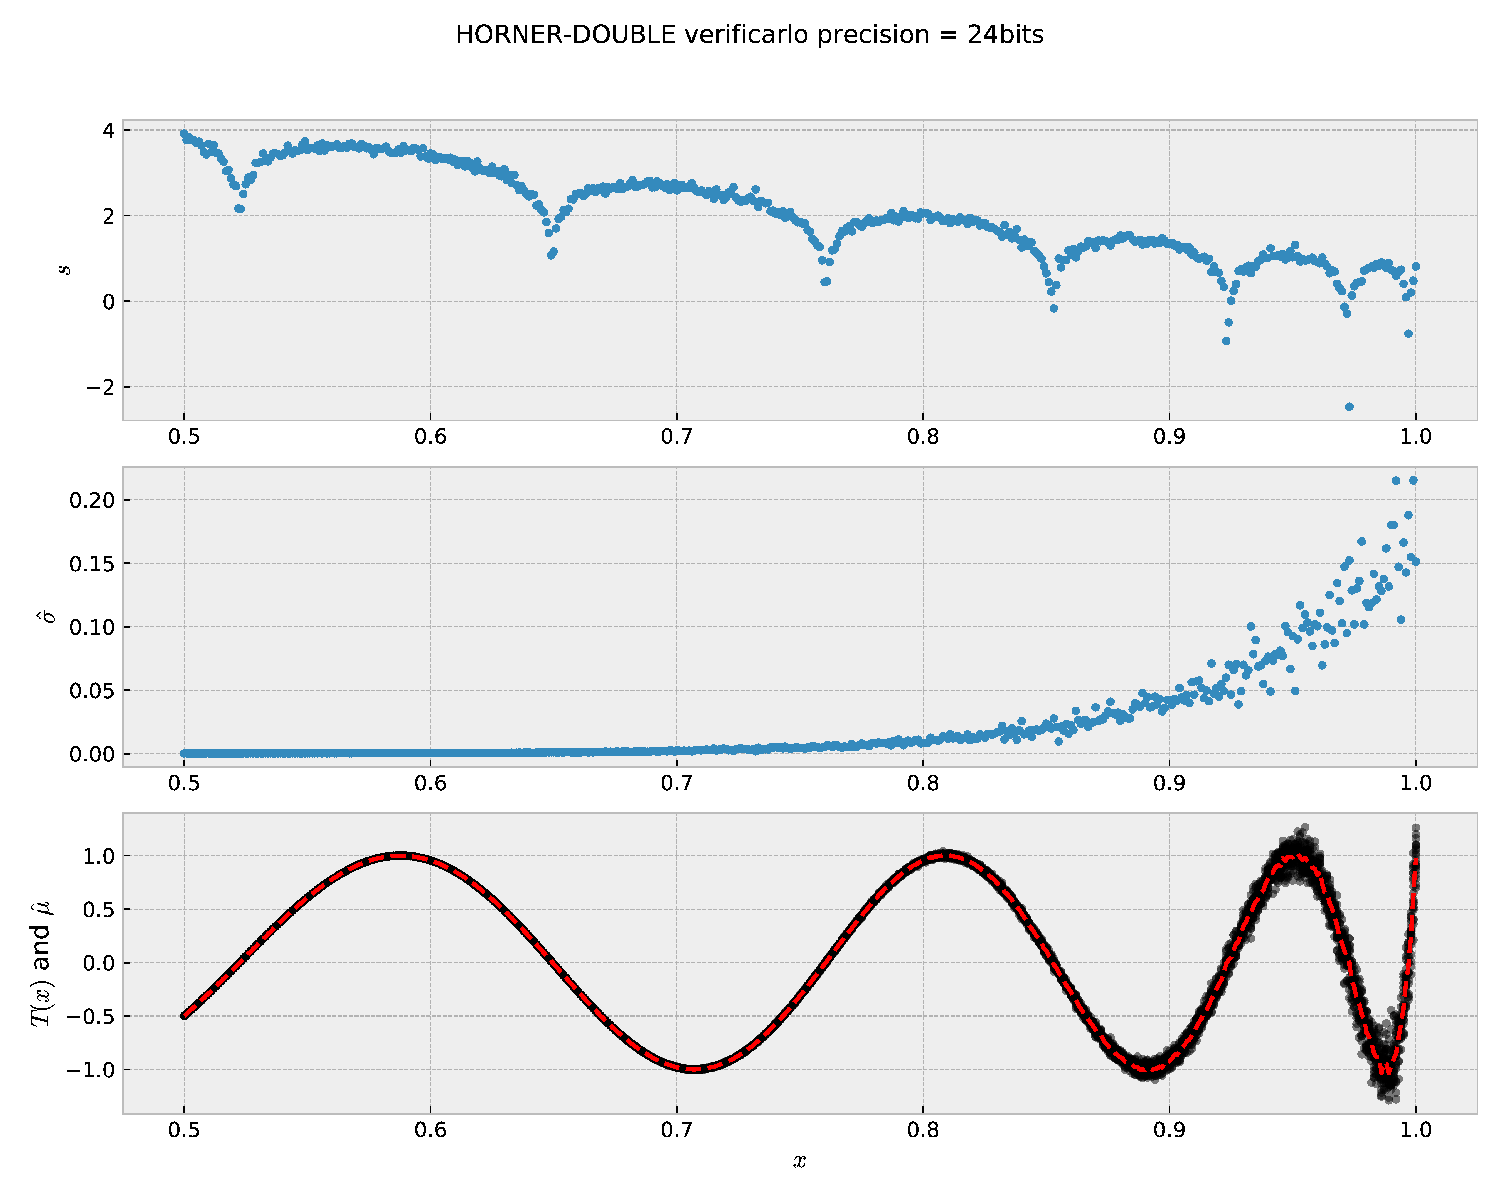
\includegraphics[width=.47\textwidth]{HORNER-DOUBLE-24.pdf} &
    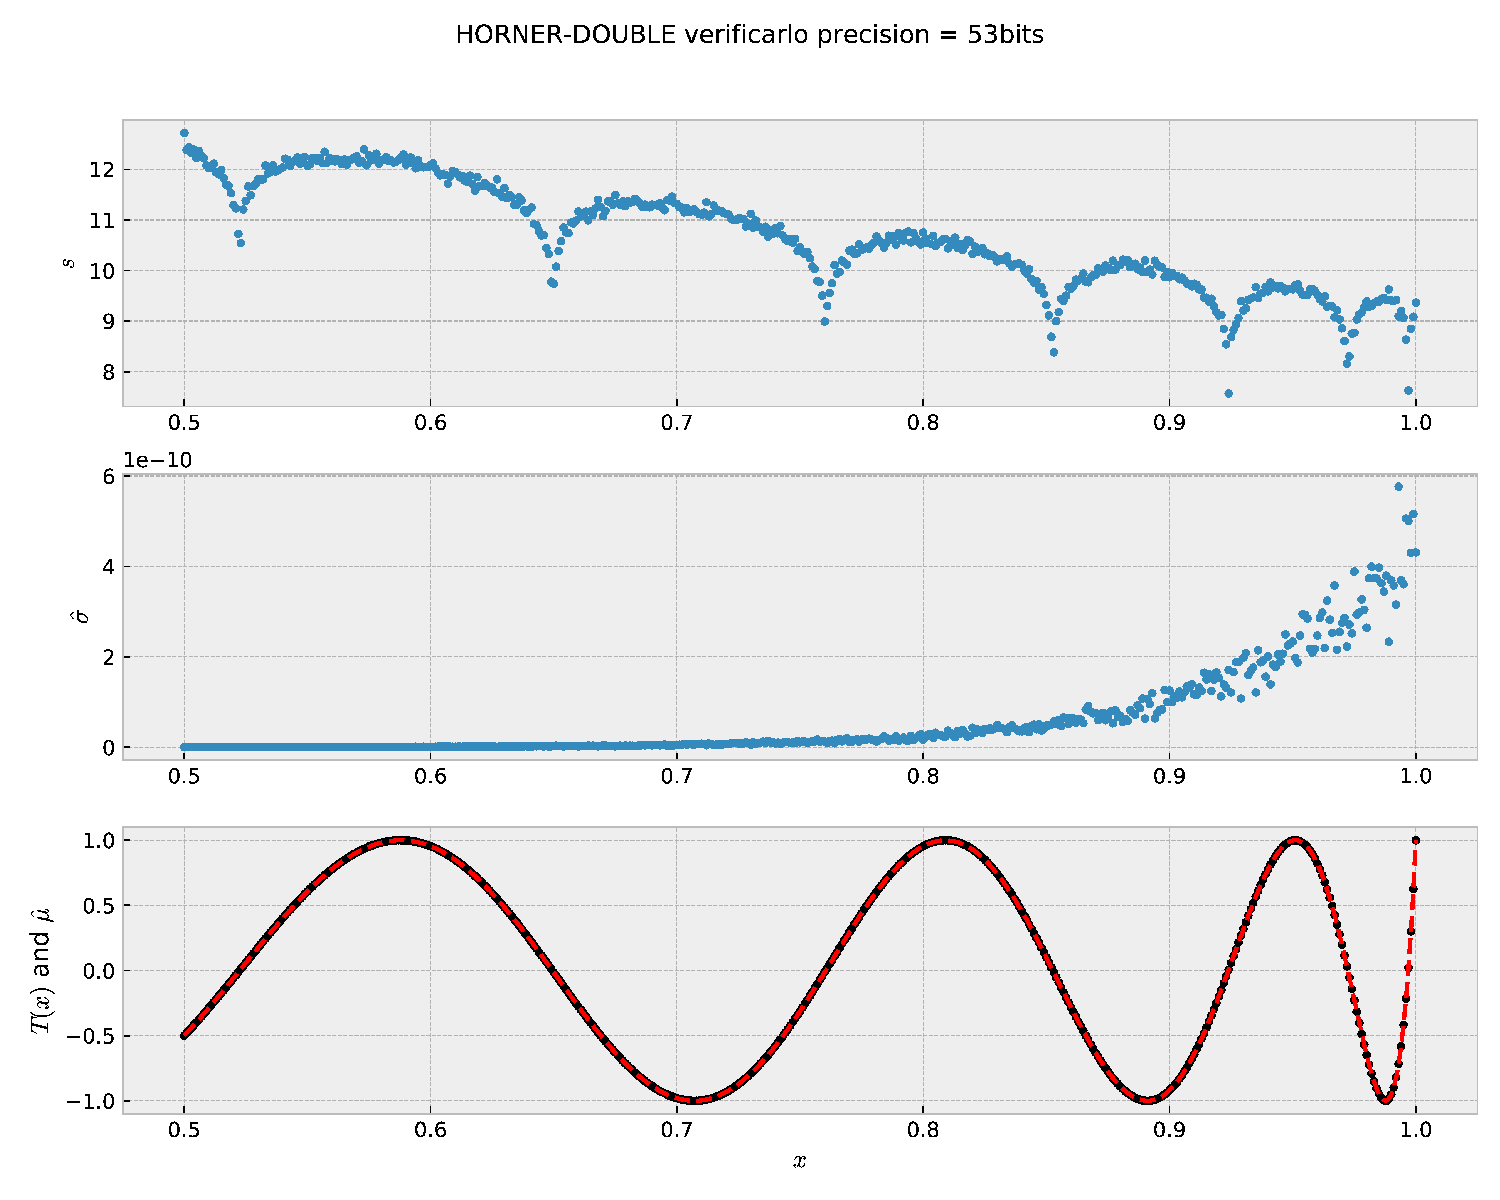
\includegraphics[width=.47\textwidth]{HORNER-DOUBLE-53.pdf}   \\
    %Horner form, 24 bits & Horner form, 53 bits \\
  \end{tabular}
  \caption{Evaluation of T(x) with Horner's scheme, compiled in double precision, with a virtual precision of \{24/53\} bits}
  \label{fig:hor_24_53}
\end{table}



As shown in this experiment, the improvment brought by the Horner scheme is not significant ($\simeq$ 1 additional significant bit in the result).
However, it minimizes the
number of operations and allows to use the FMA ({\it Fused Multiply Add}). For
a polynomial of degree $n$, it produces $n-1$ FMA. Moreover, when doing
multiple independent evaluations it can be vectorized.

\subsection{Compensated Horner's method}

\emph{Compensated} algorithms belong to the class of algorithms that increase
program precision without changing the internal working format.
The goal is to capture for each operation an estimation of the error term and to reinject it into the result.
For the Horner scheme, it is possible to retrieve at every step the error in
$x^2$ and the addition of the next coefficient by using respectively the
$Veltkamp-Dekker$ {\tt TWOPROD} for the product and { \tt TWOSUM } for the sum.
These algorithms are qualified as ({\it Error Free Transform}), EFT, in the
literature.
The algorithm for the compensated horner scheme described in \cite{graillat2005compensated} is:

\begin{algorithmic}[1]
  \Procedure{compHorner}{$x$,$\{a_1, a_2, \ldots, a_n\}$}
  \State {$s_n \gets a_n$}
  \State {$r_n \gets 0$}
  \For {$i \in [n-1:0]$}
  \State $[p_i, pe_i] \gets \text{\sc TWOPROD}(s_{i+1}, x^2)$
  \State $[s_i, se_i] \gets \text{\sc TWOSUM}(p_i, a_i)$
  \State $r_i \gets r_{i+1}\times x^2+(pe_i+se_i)$
  \EndFor
  \State \Return $s_0 + r_0$
  \EndProcedure
\end{algorithmic}

The lines 5 and 6, evaluate HORNER with EFT calls. Line 7 accumulates the error terms, which will be added to the final result in line 9.

We provide implementations for EFT in the {\tt libeft.c} and {\tt libeft.h} files.

\begin{question}
  \begin{enumerate}[(a)]
    \item Implement comphorner algorithm in {\tt tchebychev.c} using the EFT implementations in {\tt eft.h}.
    \item Modify {\tt run.sh} to also compile eft.c with verificarlo.
    \item Run comphorner with the following command: {\tt ./run.sh COMPHORNER FLOAT 24 rr}
    \item Run comphorner with the following command: {\tt ./run.sh COMPHORNER DOUBLE 53 rr}
    \item What happens if you use a precision different from 53 for program compiled in DOUBLE precision?
          $\Rightarrow$ WARNING, {\sc TWOPROD} and {\sc TWOSUM} rely on exact operations; it is essential to use RR 53 (Random Rounding with precision 53) mode of verificarlo for  \texttt{double} or RR 24 for \texttt{float}.
          \\~\\
          You should get results shown in figure~\ref{fig:comphornerVerificarlo24_53}.

  \end{enumerate}
\end{question}


\begin{table}
  \begin{tabular}{cc}
    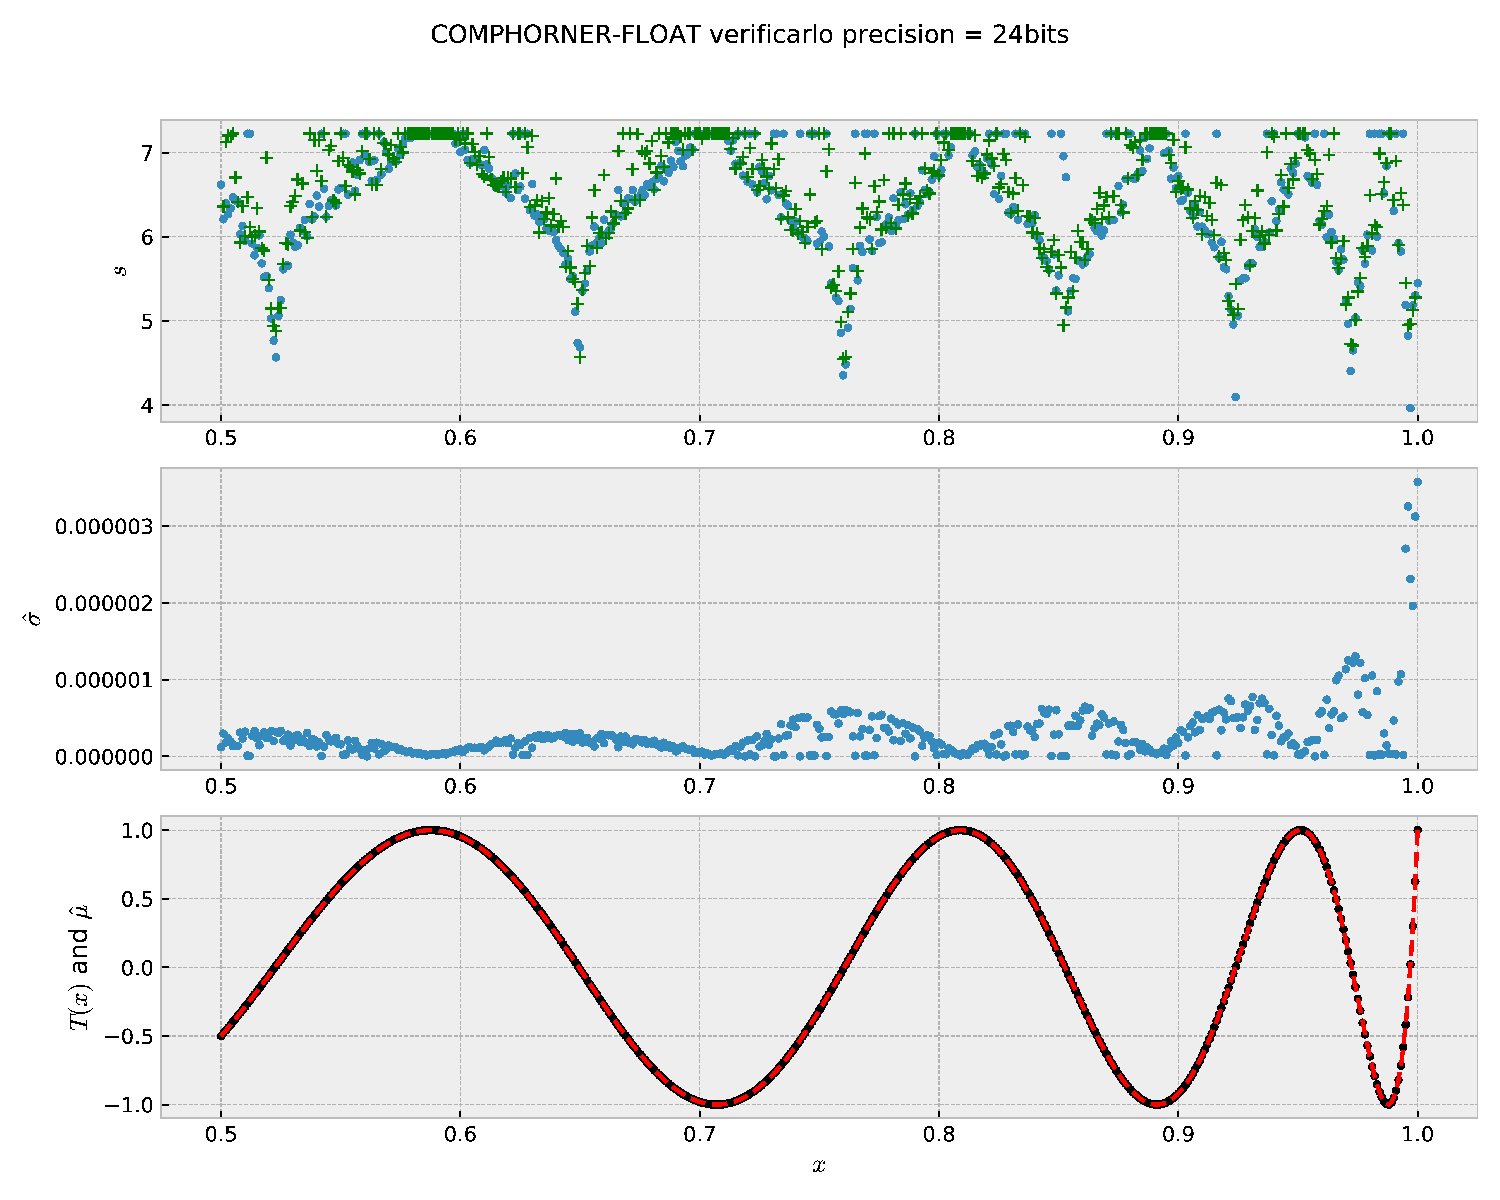
\includegraphics[width=.47\textwidth]{COMPHORNER-FLOAT-24+err.pdf} &
    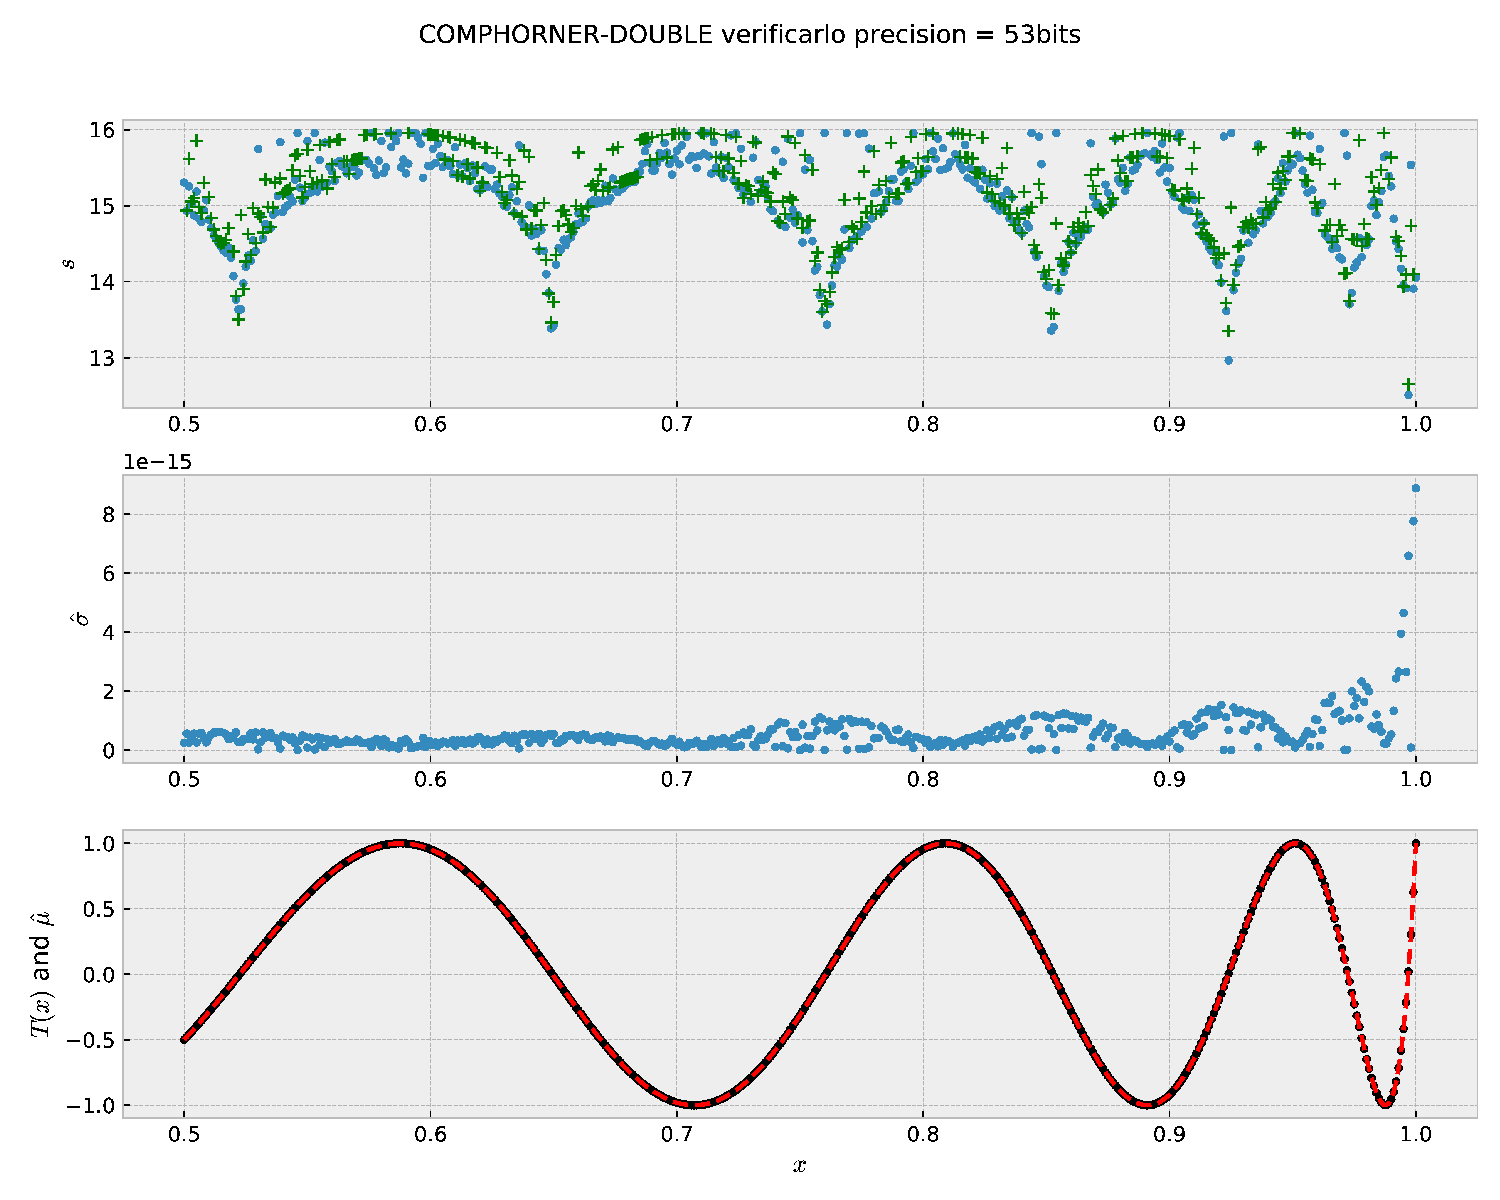
\includegraphics[width=.47\textwidth]{COMPHORNER-DOUBLE-53+err.pdf}  \\
  \end{tabular}
  \caption{Evaluation of T(x) using Horner and compHorner in single/double (left/right) precision: error estimated by verificarlo (blue), compared to the real error (green)}
  \label{fig:comphornerVerificarlo24_53}
\end{table}


The resulting precision of this approach is shown in table~\ref{fig:comphornerVerificarlo24_53} with verificarlo.
Filled circles represent the real error value (evaluating in rational arithmetic in Python); circles represent the quality of the result computed in Monte Carlo Arithmetic with Verificarlo~\cite{verrou}.

We can notice on these figures that CompHorner compensate precision losses in double and single precision. We retrieve a behavior similar to the factored form, in particularly for points $T(x)=1$. However, knowing the polynomial's roots for using the Horner scheme is not required.

%Out of these plots, we can make two interesting observations.
%First, at the cost of an increasing number of operations, (but generally in the same complexity class) it is possible to recover a part (or the full) precision losses. There are algorithms called "accurate" that compute result without loss of precision, by, for example, recursively keeping errors terms until they can not be represented in the final result and such that rounding is correct ({\it e.g.} $accSum$ of S. Rump).
%
%Second, some algorithms, especially in mathematical libraries (libmath, Intel MKL, Intel VML, libeft) exploit particularities of the floating-point format. By using Monte Carlo Arithmetic, it can be difficult to analyze them. In the RR mode, a large amount of compensated algorithms can be analyzed (including compHorner as seen before). In addition, by their design, most of these algorithms have a proof of their level's precision correctness, which makes their evaluation by empirical methods less interesting for error bounds extimation, but is still relevant to characterize the error distribution.
